\documentclass{beamer}
\usepackage[italian]{babel}
\usepackage{multicol}

\usepackage{tikz}
\usepackage{graphicx}
\usepackage[table, x11names]{xcolor}
\usepackage{xstring}
\usepackage{etoolbox}
\usepackage{multirow}
\usepackage{tabularx}
\usepackage[export]{adjustbox}
\usepackage[font=tiny]{caption}

\newcommand{\Date}{}

\newcommand{\setDate}[1]{\renewcommand{\Date}{#1}}

\useinnertheme{default}
\useoutertheme{default}
\usecolortheme{default}

\definecolor{aziendaPrimary}{RGB}{84, 150, 104}
\setbeamercolor{structure}{fg=aziendaPrimary}
\setbeamercolor{frametitle}{bg=aziendaPrimary!10,fg=aziendaPrimary}

% rimuovere i simboli di navigazione
\setbeamertemplate{navigation symbols}{}


% pagina iniziale
\setbeamertemplate{title page}{
  \vspace{4em}
  \begin{center}
    \hspace{1.5cm}
    \begin{minipage}{0.3\textwidth}
      \centering
      
\includegraphics[height=2.5cm, right]{../logo-crop.pdf}
    \end{minipage}
    \begin{minipage}{0.3\textwidth}
      \centering
      
\includegraphics[height=2.5cm, left]{img/logounipd.png}
    \end{minipage}
  \end{center}
  \begin{center}
    \vspace{0.5em}
      {\usebeamerfont{title}\color{black}\textbf{\inserttitle}\par}
    \vspace{0.7em}
    {\usebeamerfont{date}\insertauthor\par}
    \vspace{0.5cm}
    {\usebeamerfont{date}\Date\par}
  \end{center}
}

% footer
\setbeamertemplate{footline}{
  \vspace{2ex}
  \hbox{
    \begin{minipage}[t]{0.40\paperwidth}
      \hspace*{0.5em}
      \raggedright\usebeamerfont{footline}{Presentazione architettura 20/04/2026}
    \end{minipage}%
    \begin{minipage}[t]{0.20\paperwidth}
      \centering\usebeamerfont{footline}Slide \insertframenumber{} di \inserttotalframenumber
    \end{minipage}%
    \begin{minipage}[t]{0.40\paperwidth}
      \hfill
      \insertshortauthor
      \hspace*{0.8em}
      \raisebox{-0.25\height}{
\includegraphics[width=0.7cm]{../logo-crop.pdf}}
      \hspace*{1.3em}
    \end{minipage}
  }
  \vspace{0.8ex}
}

\usepackage[absolute,overlay]{textpos}

\title{Presentazione PB}
\author[]{Gruppo 1 - A.A 2025/2026}
\setDate{22/04/2026}

\begin{document}
{
\setbeamertemplate{footline}{}
\begin{frame}
  \titlepage
\end{frame}
}

\begin{frame}{Stato completamento del prodotto (1/2)}
  \begin{figure}
  \centering
    \normalsize
    \begin{tabular}{|c|c|c|c|c|}
      \hline
      \cellcolor{aziendaPrimary!20}\textbf{Tipologia} & \cellcolor{aziendaPrimary!20}\textbf{Obbligatori}
                                                      & \cellcolor{aziendaPrimary!20}\textbf{Desiderabili} & \cellcolor{aziendaPrimary!20}\textbf{Opzionali}
                                                      & \cellcolor{aziendaPrimary!20}\textbf{Totali}                                                                                                 \\
      \hline
      Funzionali                                      & 85/85                                                 & 10/10                                              & 8/10   & 103/105                      \\
      \hline
      Di qualità                                      & 12/12                                                 & 0/0                                               & 7/9       & 19/21                           \\
      \hline
      Di vincolo                                      & 3/3                                                  & 4/5                                               & 0/2        & 7/10                            \\
      \hline
      \cellcolor{aziendaPrimary!20}\textbf{Totali}    & 100/100                                                & 14/15                                              & 15/21    & \cellcolor{aziendaPrimary!20} 129/136  \\
      \hline
    \end{tabular}
    \caption{Rapporto tra il numero di requisiti soddisfatti e totali.}
  \end{figure}
% \begin{center}
%     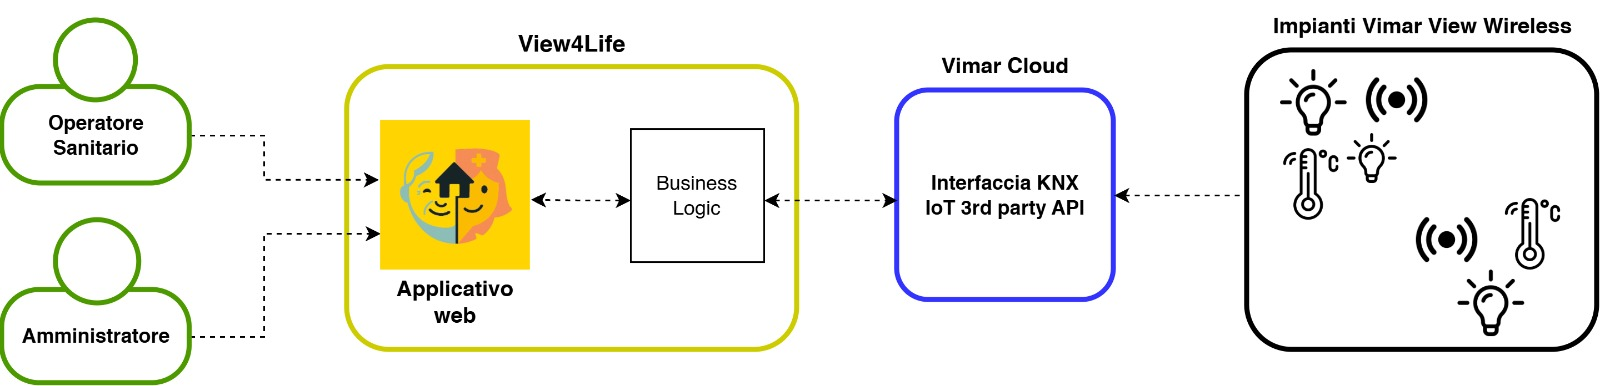
\includegraphics[width=0.95\textwidth]{img/schemacapitolato.jpeg}\\
% \end{center}
\end{frame}

\begin{frame}{Stato completamento del prodotto (2/2)}
  \begin{figure}
  \centering
    \footnotesize
    \begin{tabular}{|c|c|c|c|c|}
      \hline
      \cellcolor{aziendaPrimary!20}\textbf{Componente} & \cellcolor{aziendaPrimary!20}\textbf{Unità}
                                                      & \cellcolor{aziendaPrimary!20}\textbf{Integrazione} & \cellcolor{aziendaPrimary!20}\textbf{End-to-End}
                                                      & \cellcolor{aziendaPrimary!20}\textbf{Media totale}                                                                                                 \\
      \hline
      Backend                                      & 92,68\%                                                 & 92,91\%                                             & \multirow{3}{*}{80,18\%}   & 88,59\% \\ 
      \cline{1-3} \cline{5-5}
      Frontend                                      & 89,75\%                                                & 90,14\%                                               &       & 86,69\%                           \\
      \cline{1-3} \cline{5-5}
      \cellcolor{aziendaPrimary!20}\textbf{Media totale}    & 91,21\%                                                & 91,52\%                                              &     & \cellcolor{aziendaPrimary!20} \textbf{87,64\%}  \\
      \hline
    \end{tabular}
    \caption{Percentuale di \textit{coverage} dei test di unità, integrazione ed \textit{end-to-end}}
  \end{figure}
\end{frame}

\begin{frame}{Esito colloquio Prof. Cardin}
\begin{itemize}
  \item Attenzione che bisogna definire una autovalutazione, non cosa ci ha detto lui
\end{itemize}
\end{frame}

\end{document}